\documentclass[12pt,a4]{article}
\usepackage[english]{babel}
\usepackage[utf8]{inputenc}
\usepackage[T1]{fontenc}
\usepackage{geometry}
\usepackage{float}
\geometry{
	a4paper,
	left=20mm,
	right=20mm,
	top=20mm,
	bottom=20mm,
}
% Useful packages
\usepackage{amsmath}
\usepackage{bm}
\usepackage{graphicx}
\usepackage[colorlinks=true, allcolors=blue]{hyperref}

\begin{document}


\section{Linear Control of the Otter}
This document describe the steps taken in order to go from a nonlinear 6 DOF model of the Otter to a linear 3 DOF model.
The 3 DOF model is then used to control the Otter.
\section{The Otter}
The Otter is a small unmanned surface vehicle (USV) made by Maritime Robotics. It is a twin-hull vessel measuring 200cm x 108cm x 81.5cm and weighing 55 kg.
The Otter is used as a the subject of control in this project. The main reason for using the otter is that differential equations of the vessel could be obtained from the
\href{https://github.com/cybergalactic/MSS/blob/master/VESSELS/otter.m}{MSS toolbox}, a toolbox written by Thor I. Fossen. These equations describe the movement of the vessel in 6 degrees of freedom (6 DOF). In control they are more commonly know as the system equations, and obtaining these is fundamental to control. The system equations of a vessel like the otter can be very cumbersome to obtain as one has to account for the hydrodynamics that influence the movement of the vessel.
\begin{figure}[H]
	\centering
	\includegraphics[width = 0.8\textwidth]{graphics/theOtter.png}
	\caption{The Otter ASV}
	\label{fig:theOtter}
\end{figure}

\subsection{The system equations}
The dynamic of a vessel can be described as follows, using a 6 DOF model.
\begin{align}
	\label{eq:standard_nu}
	\bm{M}_{RB}\bm{\dot{\nu}} + \bm{M}_{A}\bm{\dot{\nu_r}} + \bm{C}_{RB}(\bm{\nu})\bm{\nu} + \bm{C}_{A}(\bm{\nu}_r)\bm{\nu}_r
	+ \bm{D}(\bm{\nu}_r)\bm{\nu}_r +\bm{G}\bm{\eta} & = \bm{\tau} + \bm{w}(t) \\
	\bm{\dot{\eta}}                                 & = \bm{J}(\eta)\bm{\nu}
\end{align}
where $\nu$ is the velocities and $\eta$ is the positions. This description includes a velocity and a position in each of the 6 modes.
The modes are translation in x, y and z and rotation around x, y and z. $\nu_r$ is the relative speed of the vessel to the water.

In the model from the MSS toolbox the system equations are given as
\begin{align}
	\label{eq:MSS_nu}
	{\dot{\nu}}  & = \frac{\tau + \tau_{damp} + \tau_{crossflow} - C \nu_r - G \eta - g_0}{M} \\
	{\dot{\eta}} & =   J(\eta) \nu
\end{align}

Expanding (\ref{eq:MSS_nu}) we get a set of 6 coupled differential equations. The equations for surge speed $u$, sway speed $v$ and yaw rate $r$ is shown here.
\begin{multline}
	\dot{u} = 0.0054\,\tau _{q}-1.3169\,q+0.0175\,\tau _{u}+0.00053523\,\tau _{w}-16.0798\,\theta \\-1.3574\,u-0.2925\,w-12.1092\,z+0.3371\,p\,r-0.0147\,p\,v-0.0265\,q\,u-1.8664\,q\,w\\+2.3477\,r\,v+0.2649\,u\,w+0.0177\,p^2+0.1866\,q^2+0.1690\,r^2
\end{multline}
\begin{multline}
	\dot{v} = 0.2504\,p+4.9601\,\phi +0.0667\,r-0.0046\,\tau _{p}-0.0014\,\tau _{r}+0.0078\,\tau _{v}\\-0.00059306\,v-0.0364\,p\,q+0.1167\,q\,r+0.7867\,p\,w-0.4028\,r\,u-0.1266\,v\,w+0.3298\,r\,\left|r\right|\\+0.1143\,r\,\left|v\right|-0.9463\,v\,\left|v\right|
\end{multline}
\begin{multline}
	\dot{r} = 0.2696\,p+5.3406\,\phi -1.0413\,r-0.0050\,\tau _{p}+0.0229\,\tau _{r}-0.0014\,\tau _{v}\\+0.0013\,v-0.4188\,p\,q+0.1257\,q\,r+0.0395\,p\,w-0.1107\,r\,u-0.1363\,v\,w-10.3735\,r\,\left|r\right|\\-2.0239\,r\,\left|v\right|+0.1699\,v\,\left|v\right|
\end{multline}



\section{Modelling}
\subsection{3 DOF}
Making a 3 DOF model using only surge, sway and yaw, is simply a matter of discarding the 3 differential equations that describe the behaviour of the other modes.
In the remaining 3 differential equations heave, roll and pitch is assumed to be zero. That is $w = 0$, $p=0$ and $q = 0$.
Doing this yields
\begin{equation*}
	\dot{u} = 0.1690\,r^2+2.3477\,v\,r+0.0175\,\tau _{u}-1.3574\,u
\end{equation*}
\begin{equation*}
	\dot{v} = 0.0736\,r-0.0014\,\tau _{r}+0.0078\,\tau _{v}-0.0949\,v-0.4028\,r\,u+0.6506\,r\,\left|r\right|
\end{equation*}
\begin{equation*}
	\dot{r} = 0.0229\,\tau _{r}-1.1746\,r-0.0014\,\tau _{v}+0.0176\,v-0.1107\,r\,u-10.3762\,r\,\left|r\right|
\end{equation*}
The same is done for $\dot{\eta}$, resulting in
\begin{equation*}
	\dot{x} = u\,\cos\left(\psi \right)-v\,\sin\left(\psi \right)
\end{equation*}
\begin{equation*}
	\dot{y} = v\,\cos\left(\psi \right)+u\,\sin\left(\psi \right)
\end{equation*}
\begin{equation*}
	\dot{\psi} = r
\end{equation*}
This clearly describe a simple transformation of the velocities. The transformation is a rotation around the z-axis by $\psi$.
The system equations of the 3 DOF model is then define as
\begin{align}
	\bm{f}_\nu = \bm{\dot{\nu}(x)}   & = \begin{bmatrix} \dot{u} \\ \dot{v} \\ \dot{r} \end{bmatrix} &
	\bm{f}_\eta = \bm{\dot{\eta}(x)} & = \begin{bmatrix} \dot{x} \\ \dot{y} \\ \dot{\phi} \end{bmatrix}
\end{align}


\subsection{State space representation}
Having the system equations, the state space representation of the velocities $\nu$
\begin{equation}
	\bm{\dot{\nu}} = \bm{A \nu} + \bm{B \tau}
\end{equation}
can be made by calculating the following Jacobian matrices
\begin{align}
	\bm{A} & = \dfrac{d\bm{f}_\nu}{d\bm{\nu}} & \bm{B} & = \dfrac{d\bm{f}_\nu}{d\bm{\tau}}
\end{align}
And evaluating them at a certain linearization point. The Jacobian matrices are
\begin{equation}
	\bm{A} =     \left[\begin{array}{ccc} -1.3574 & 2.3477\,r & 0.3379\,r+2.3477\,v\\ -0.4028\,r & -0.0949 & 1.3012\,\left|r\right|-0.4028\,u+0.0736\\ -0.1107\,r & 0.0176 & -0.1107\,u-20.7524\,\left|r\right|-1.1746 \end{array}\right]
\end{equation}
\begin{equation}
	\bm{B}    =     \left[\begin{array}{ccc} 0.0175 & 0 & 0\\ 0 & 0.0078 & -0.0014\\ 0 & -0.0014 & 0.0229 \end{array}\right]
\end{equation}

If we choose the linearization point $u = 3\,$kn, $v = 0$ and $r = 0$, which is a simple forward movement. The state-space representation becomes
\begin{equation}
	\bm{A} = \left[\begin{array}{ccc} -1.3574 & 0 & 0\\ 0 & -0.0949 & -0.5480\\ 0 & 0.0176 & -1.3454 \end{array}\right]
\end{equation}
The matrix $\bm{B}$ does of course not change, as it is not depending on the state.


\section{Control}
\subsection{Control Allocation}
Before designing a controller we need to address a problem with the linear state space model. This model takes a vector of control forces $\tau$ as input.
Making a controller for this system will result in a controller that provides $\tau$ as the input to the Otter.
However the Otter will need to know to how position its propellers and fast they should spin, not what the resulting force should be.
\subsubsection{Dynamics of the propellers}
First we can split $\tau$ into linear force and torque.
\begin{equation}
	\bm{\tau} = \begin{bmatrix}
		\bm{\tau}_{linear} \\
		\bm{\tau}_{torque}
	\end{bmatrix}
\end{equation}
If we define the force $T$ provided by a propeller as a vector in the vessels coordinate frame (surge, sway, heave).
\begin{equation}
	\bm{T} = \begin{bmatrix} F_u \\ F_v \\ F_w \end{bmatrix}
\end{equation}
The linear control force is found as the sum of forces from each propeller p.
\begin{equation}
	\bm{\tau}_{linear} = \sum^P \bm{T}_p
\end{equation}
While the torque of each propeller can be found as the cross product between the force $\bm{T}_p$ and the position at which it acts $\bm{r}_p$.
The total torque is then the sum of torques from the propellers.
\begin{equation}
	\bm{\tau}_{torque} = \sum^P  \bm{r}_p \times \bm{T}_p = \sum^P S(\bm{r}_p) \bm{T}_p
\end{equation}
$\bm{r}_p$ is simply the position vector of thruster \textit{p} and $S(\bm{r}_p)$ is the skew-symetric matrix of vector $\bm{r}_p$
which simplify the cross product operation. In the case of two propellers we have
\begin{equation}
	\bm{\tau}_{linear} = \bm{T}_1 + \bm{T}_2
\end{equation}
\begin{equation}
	\bm{\tau}_{torque} = S(\bm{r}_1)\bm{T}_1+ S(\bm{r}_2)\bm{T}_2
\end{equation}
Which can be written as
\begin{equation}\label{eq:CA_matrix}
	\bm{\tau} = \begin{bmatrix}		\bm{\tau}_{linear} \\		\bm{\tau}_{torque}	\end{bmatrix}
	=\begin{bmatrix} \bm{I} & \bm{I} \\ S(\bm{r}_1) & S(\bm{r}_2) \end{bmatrix}\begin{bmatrix} \bm{T}_1 \\ \bm{T}_2 \end{bmatrix}
\end{equation}

Each propeller can rotate with an angle $\xi_p$. The thrust of each propeller can be describe as a vector by splitting it into components that align with the vessels coordinate frame
\begin{equation}
	\bm{T}_p = \begin{bmatrix} \cos(\xi_p)\\ \sin(\xi_p)\\ 0 \end{bmatrix} t_p
\end{equation}
where $t_p$ is the magnitude of the thrust from each propeller and $\bm{T}_p$ is the resulting force vector. This is done under the assumption that the propellers are only able to move in the horizontal plane, hence $F_w = 0$. If roll and/or pitch is included in the model, this should be adjusted accordingly.
The last thing that is needed is the relationship between the thrust and the revolutions of the propeller. From [Mogens] this relationship is
\begin{equation}\label{eq:CA_thrust}
	t_p = T_{nn}n_p^2+T_{nv}V_A n_p \quad,\quad T_{nn} > 0 > T_{nv}
\end{equation}
Where $T_{nn}$ and $T_{nv}$ are scalar constants, $n_p$ is the revolutions of the propellers and $V_A$ is the apparent water velocity at the location of the propeller.
$T_{nn}$ and $T_{nv}$ can be estimated from the psysical dimensions of the propeller.

\subsubsection{Control allocation}
The problem at hand is to find $\bm{\xi}$ and $\bm{n}$ given $\bm{\tau}$. First we can find the individual force vectors of each propeller from (\ref{eq:CA_matrix})
\begin{equation}
	\begin{bmatrix} \bm{T}_1 \\ \bm{T}_2 \end{bmatrix} =
	\begin{bmatrix} \bm{I} & \bm{I} \\ S(\bm{r}_1) & S(\bm{r}_2) \end{bmatrix}^+ \bm{\tau}
\end{equation}
Where + denotes the pseudo inverse. Then, for each of the propellers, the angle and the magnitude of the thrust is found as
\begin{align}
	\xi_p & = \text{atan2}(F_v,F_u) \\
	t_p   & = \|\bm{T}_p\|
\end{align}
This will produce $\xi_p \in [\pi ; -\pi)$. However the propeller is limited to $\xi_p \in [\frac{\pi}{2} ; -\frac{\pi}{2})$,
In the case where $\xi_p$ is outside this interval we can simply turn it by $\pi$ and flip the sign on $t_p$. This will happen when a force in the aft direction is required e.g. when the vessel is moving forwards and propellers need to stop it. Turning the propeller by $\pi$ and flipping the sign on $t_p$ is analogous to putting the propellers in reverse.
Finally the required revolutions can by calculated as
\begin{equation}
	n_p = \text{sgn}(t_p) \dfrac{\sqrt{Tnv^2 V_A^2 + 4 T_{nn} |t_p|}-T_{nv} V_A}{2 T_{nn}}
\end{equation}
This expression is found by solving (\ref{eq:CA_thrust}) for $n_p$. Notice that the term under the square root will always be positive as $T_{nn}>0$.
Finally we can stack the result in vectors.
\begin{align}
	\bm{\xi} & = \begin{bmatrix} \xi_1 \\ \xi_2 \end{bmatrix} & \bm{n} & = \begin{bmatrix} n_1 \\ n_2 \end{bmatrix}
\end{align}
This

\subsection{Kinematics}
The dynamic of a vessel can be described as follows, using a 6 DOF model.
\begin{align}
	\bm{M}_{RB}\bm{\dot{\nu}} + \bm{M}_{A}\bm{\dot{\nu_r}} + \bm{C}_{A}(\bm{\nu})\bm{\nu} + \bm{C}_{RB}(\bm{\nu}_r)\bm{\nu}_r
	+ \bm{D}(\bm{\nu}_r)\bm{\nu}_r +\bm{G}\bm{\eta} & = \bm{\tau} + \bm{w}(t) \\
	\bm{\dot{\eta}}                                 & = \bm{J}(\eta)\bm{\nu}
\end{align}
where $\nu$ is the velocities and $\eta$ is the positions. This description includes a velocity and a position in each of the 6 modes.
The modes are translation in x, y and z and rotation around x, y and z. $\nu_r$ is the relative speed of the vessel to the water

\subsection{State space}
Assuming $\nu = \nu_r$ (no movement of the water relative to the seabed), we can define

\begin{align}
	\bm{M}           & = \bm{M}_{RB} + \bm{M}_{A}                     \\
	\bm{C}(\bm{\nu}) & = \bm{C}_{RB}(\bm{\nu}) + \bm{C}_{A}(\bm{\nu})
\end{align}
And write the system as
\begin{align}
	\bm{M}\bm{\dot{\nu}} + \bm{C}(\bm{\nu})\bm{\nu} + \bm{D}(\bm{\nu})\bm{\nu} +\bm{G}\bm{\eta} & = \bm{\tau} + \bm{w}(t) \\
	\bm{\dot{\eta}}                                                                             & = \bm{J}(\eta)\bm{\nu}
\end{align}
Solving for $\bm{\dot{\nu}}$ we get
\begin{align}
	\bm{\dot{\nu}}  & =	\bm{A}(\bm{\nu})\bm{\nu}+\bm{G}\bm{\eta}+\bm{B}\bm{\tau} 		\label{eq:nu_ss} \\
	\bm{\dot{\eta}} & =	\bm{J}(\eta)\bm{\nu}								\label{eq:eta_ss}
\end{align}
Where
\begin{align}
	\bm{A}(\bm{\nu}) & = -\bm{M}^{-1}(\bm{C}(\bm{\nu})+\bm{D}(\bm{\nu})) \\
	\bm{B}           & = \bm{M}^{-1}
\end{align}
Writing (\ref{eq:nu_ss}) and (\ref{eq:eta_ss}) in matrix form gives us a state space description of the whole system

\begin{equation}
	\bm{\dot{x}} =	\begin{bmatrix} \bm{A}(\bm{\nu}) & \bm{G} \\ \bm{J}(\eta) & \bm{0} \end{bmatrix}\bm{x}
	+ \begin{bmatrix}	\bm{B} \\ \bm{0}	\end{bmatrix}\bm{\tau}
\end{equation}
where
\begin{equation}
	\bm{x} = \begin{bmatrix} \bm{\nu}\\ \bm{\eta} \end{bmatrix}
\end{equation}
\begin{align}
	\bm{\nu}  & = \begin{bmatrix} u \\ v \\ w \\ p \\ q \\ r \end{bmatrix}
	          &
	\bm{\eta} & = \begin{bmatrix} x \\ y \\ z \\ \phi \\ \theta \\ \psi \end{bmatrix}
\end{align}


\section{Measurements}
The vessel is fitted with a satellite compass and GPS like the one seen in figure \ref{fig:Furuno_SC70}. This device can provide the following data
\begin{table}[H]
	\centering
	\begin{tabular}{c|l}
		SoG & Speed over Ground also know as track \\
		CoG & Course over Ground                   \\
		RoT & Rate of Turn (in yaw)                \\
		Pos & Position of vessel in x and y        \\
		HDT & Heading of vessel
	\end{tabular}
\end{table}
\begin{figure}[H]
	\centering
	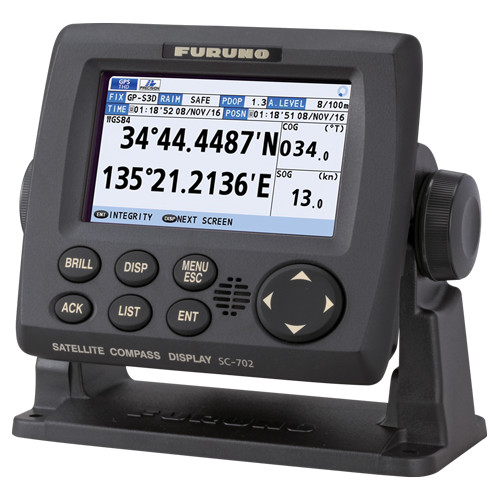
\includegraphics[width = 0.5\textwidth]{graphics/Furuno SC70.jpg}
	\caption{Furuno SC70. Differential GPS (DGPS) and compass}
	\label{fig:Furuno_SC70}
\end{figure}
Assuming normal noise distribution the measurement equations can be written as

\begin{align}
	HDT & = \psi + w                                    \\
	Pos & = \begin{bmatrix} x \\ y \end{bmatrix} + w              \\
	SoG & = \left|\begin{bmatrix} u \\ v \end{bmatrix}\right| + w \\
	CoG & = atan2(v,u) + w                              \\
	RoT & = r + w
\end{align}

\begin{align}
	\bm{y}   & = \bm{C}_m \bm{x} \\
	\bm{C}_m & = \bm{I}
\end{align}

\section{Control}
\begin{figure}[H]
	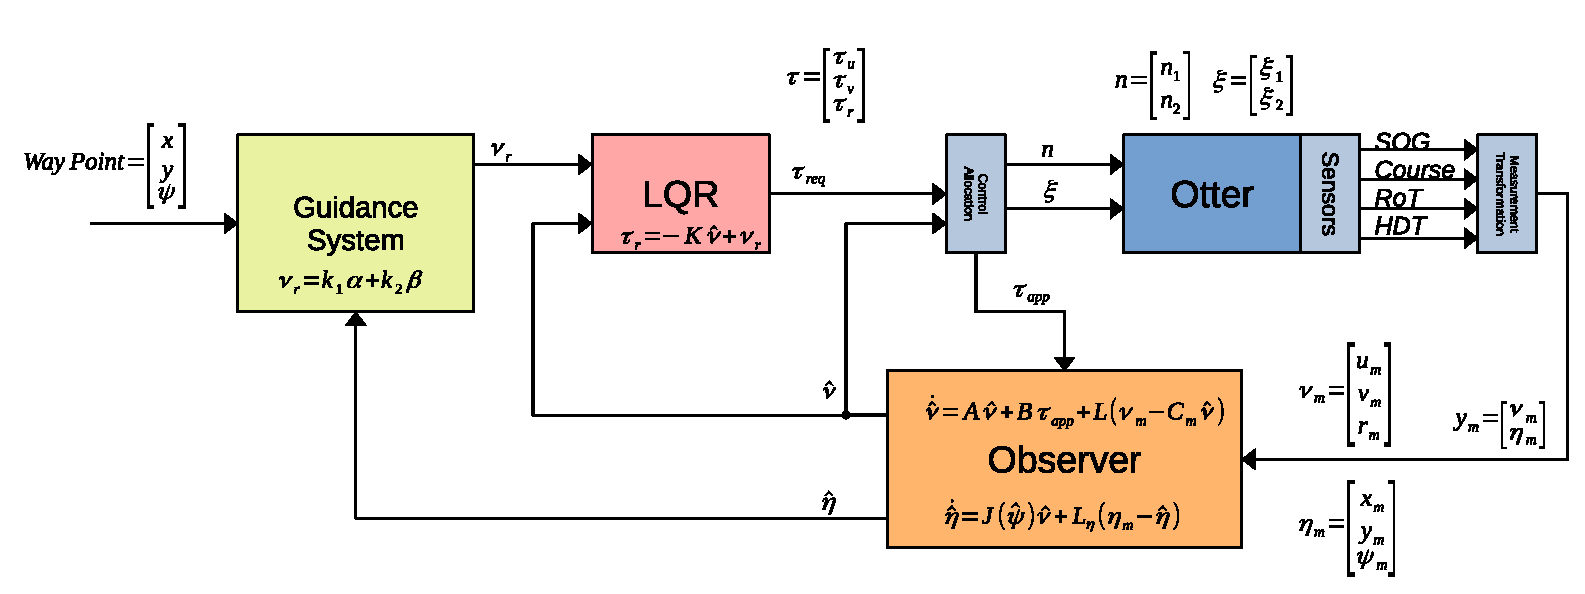
\includegraphics[width = \textwidth]{graphics/BlokDiagram.eps}
	\caption{}
	\label{}
\end{figure}

\section{Observer}

\subsection{Ordinary Kalman filter}

\subsection{Adaptive Kalman filter}
Given the input $u$ and the measurement $y_m$
Data update
\begin{align*}
	S_n      & = C_m P C_m^T + R_{vv}      \\
	\kappa   & = P C_m^T S_n^{-1}          \\
	\hat{y}  & = C_m \hat{x}               \\
	\epsilon & = y_m - \hat{y}             \\
	\hat{x}  & = \hat{x} + \kappa \epsilon \\
	P        & = P - \kappa S_n \kappa^T
\end{align*}
Time update
\begin{align*}
	x & = A x + B u       \\
	P & = A P A' + R_{ww}
\end{align*}

\section{Water current}
$\bm{\nu}_r = \bm{\nu} - \bm{\nu}_c$
\begin{multline}
	\label{eq:standard_nu}
	\bm{M}_{RB}\bm{\dot{\nu}} + \bm{M}_{A}\bm{\dot{\nu}} - \bm{M}_{A}\bm{\dot{\nu}}_c + \bm{C}_{RB}(\bm{\nu})\bm{\nu}
	+ \bm{C}_{A}(\bm{\nu}_r)\bm{\nu} -  \bm{C}_{A}(\bm{\nu}_r)\bm{\nu}_c \\
	+ \bm{D}(\bm{\nu}_r) \bm{\nu} - \bm{D}(\bm{\nu}_r) \bm{\nu}_c  +\bm{G}\bm{\eta} = \bm{\tau} + \bm{w}(t)
\end{multline}


\begin{align}
	\bm{M}_{RB}\bm{\dot{\nu}} + \bm{M}_{A}\bm{\dot{\nu}_r} + \bm{C}_{RB}(\bm{\nu})\bm{\nu} + \bm{C}_{A}(\bm{\nu}_r)\bm{\nu}_r
	+ \bm{D}(\bm{\nu}_r)\bm{\nu}_r +\bm{G}\bm{\eta} & = \bm{\tau} + \bm{w}(t) \\
	\bm{\dot{\eta}}                                 & = \bm{J}(\eta)\bm{\nu}
\end{align}
Using Property 8.1 of Fossen
\begin{equation}
	\bm{M}_{RB}\bm{\dot{\nu}} + \bm{C}_{RB}(\bm{\nu})\bm{\nu} \equiv \bm{M}_{RB}\bm{\dot{\nu}_r} + \bm{C}_{RB}(\bm{\nu}_r)\bm{\nu}_r
\end{equation}
We can rewrite the system using only the relative velocity
\begin{align}
	\bm{M}_{RB}\bm{\dot{\nu}_r} + \bm{M}_{A}\bm{\dot{\nu}_r} + \bm{C}_{RB}(\bm{\nu}_r)\bm{\nu}_r + \bm{C}_{A}(\bm{\nu}_r)\bm{\nu}_r
	+ \bm{D}(\bm{\nu}_r)\bm{\nu}_r +\bm{G}\bm{\eta} & = \bm{\tau} + \bm{w}(t) \\
	\bm{\dot{\eta}}                                 & = \bm{J}(\eta)\bm{\nu}
\end{align}
\begin{equation}
	\bm{J}(\eta)\bm{\nu}_c^l = \bm{\nu}_c^g
\end{equation}
\begin{align}
	\bm{M}_{RB}\bm{\dot{\nu}_r} + \bm{M}_{A}\bm{\dot{\nu}_r} + \bm{C}_{RB}(\bm{\nu}_r)\bm{\nu}_r + \bm{C}_{A}(\bm{\nu}_r)\bm{\nu}_r
	+ \bm{D}(\bm{\nu}_r)\bm{\nu}_r +\bm{G}\bm{\eta} & = \bm{\tau} + \bm{w}(t)               \\
	\bm{\dot{\eta}}                                 & = \bm{J}(\eta)\bm{\nu}_r+\bm{\nu}_c^g
\end{align}
\end{document}
